%%%%%%%%%%%%%%%%%%%%%%%%%%%%%
%Since : 2019/04/03
%Update: 2019/04/09
% -*- coding: utf-8 -*-
%%%%%%%%%%%%%%%%%%%%%%%%%%%%%


\chapter{Excelによる統計処理2}
\setcounter{num_prac}{0}

\section{目的}

データを解析おいて重要なデータの可視化(グラフ化)の方法を学ぶ.

\section{原理}

\subsection{グラフ}

データの特徴を視覚的に把握するためにグラフを用います.
代表的なグラフの一つが前回取り扱ったヒストグラムです.
ヒストグラム以外にも様々なグラフが存在します.
今回は,折れ線グラフ,円グラフ,散布図を取り扱います.

\paragraph{棒グラフ}

棒グラフは大きさの比較に用いられます.
時間変化を把握するのに用いてはいけません.

\paragraph{折れ線グラフ}

値の時間変化の把握に用いられます.
大きさを比べる目的で折れ線グラフを使わないようにしましょう.

\paragraph{円グラフ}

割合をは把握するために用いられます.
扇型の角度は全体に対する割合を表します.
円グラフは合計で100\%にならなければなりません.

例えば,表\ref{tab:hist}

\paragraph{散布図}

データの値同士の関係性を知りたいときがあります.
値の関係性を見るために用いられます.
例として,前回の演習で用いたアヤメのがく片の長さと幅 (iris.csv)の散布図(図\ref{fig:scatter})を示します.
散布図は関係を見るデータ,例ではアヤメのがく片の長さと幅,をそれぞれ軸とします.
そして,データの組み合わせ,例ではアヤメのがく片の長さと幅,を点で表します.
例の散布図を見ると,がく片の長さが長いほど幅が太くなる傾向がありそうなことが分かります.
データそれぞれ無関係な場合は,点は垂直,水平,円に分布します.

\begin{figure}[htbp]
    \centering
    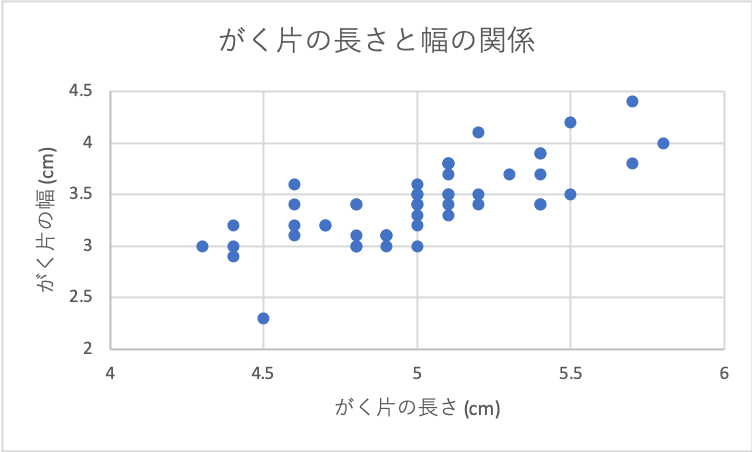
\includegraphics[width=6cm]{chap2/scatter.png}
    \caption{散布図}
    \label{fig:scatter}
\end{figure}

\paragraph{グラフに関する注意}

軸が何であるか必ず書く

\subsection{相関係数}

散布図では,視覚的に2つのデータの関係性を見ることができます.
しかし,図ではそのデータがどの程度関係しているのか定量的に分かりません.
定量的に2つのデータの関係を見る場合は相関係数を用います.
相関係数は次の式で計算されます.
\begin{equation}
    \label{eq:1}
    r = \frac{\frac{1}{N} \sum_{i=1}^N (x_i - \bar{x})(y_i - \bar{y})}{\sqrt{\frac{1}{N} \sum_{i=1}^N (x_i - \bar{x})^2} \sqrt{\frac{1}{N} \sum_{i=1}^N(y_i - \bar{y})^2}}
\end{equation}
相関係数は直線的な関係かどうかをみることができます.
相関係数が正の場合は正の相関,負の場合を負の相関と言います.
正の相関の場合,一方のデータの値が増えれば,もう一方のデータの値も増えるという関係があることが分かります.
負の相関の場合,一方のデータの値が増えれば,もう一方のデータの値は減るという関係があることが分かります.
しかし,U字型であったりS字型の関係であった場合は相関係数ではその関係性を定量化することはできません.

\subsection{散布図と回帰直線}

2つデータの値同士の関係を知るために散布図を用いる事ができることを先程述べました.
図\ref{fig:regression}のように,その関係性を直線で表したものを回帰直線と言います.
回帰直線は,データの分布を直線に近似したものです.
もう少し簡単に言えば,2つのデータの関係を直線の式$y=ax+b$に強制的に表したものです\footnote{直線近似の方法は,この講義の範疇を超えているので説明しません.興味がある人は調べてみましょう.}.

\begin{figure}[htbp]
    \centering
    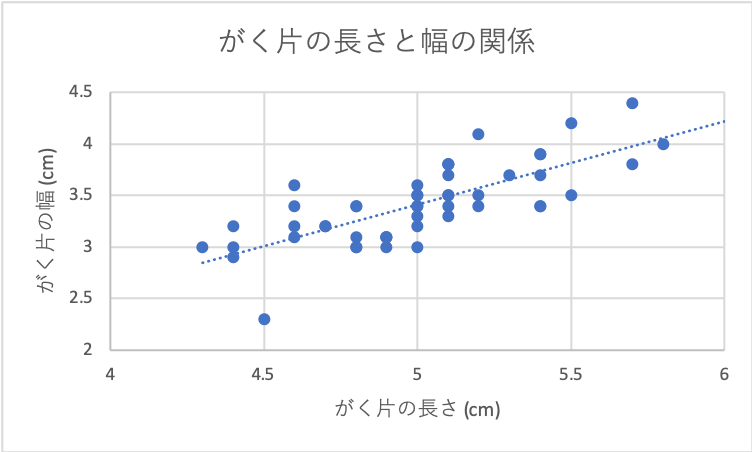
\includegraphics[width=6cm]{chap2/regression.png}
    \caption{散布図と回帰直線}
    \label{fig:regression}
\end{figure}

\section{演習}

\subsection{}


\begin{figure}[tb]
    \begin{minipage}{0.5\hsize}
        \centering
        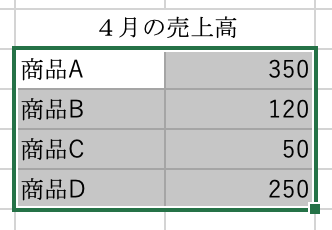
\includegraphics[width=6cm]{chap2/bar1.png}
        \caption{}
        \label{fig:bar1}
    \end{minipage}
    \begin{minipage}{0.5\hsize}
        \centering
        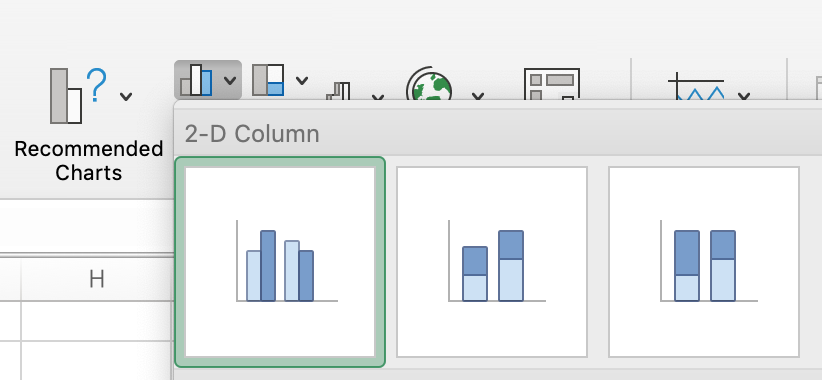
\includegraphics[width=6cm]{chap2/bar2.png}
        \caption{}
        \label{fig:bar2}
    \end{minipage}
\end{figure}


\subsection{折れ線グラフ}

手順は前回のヒストグラムと同じです.

\paragraph{演習}
csvファイルから折れ線グラフを作りなさい.ただし,横軸は 縦軸は にしなさい.

\subsection{円グラフ}

\paragraph{演習}


\subsection{折れ線グラフ}

表に示すデータを折れ線グラフにします.
横軸を,縦軸をとします.
よく軸のデータと縦軸のデータを選びます.
グラフの散布図の折れ線グラフを選びます.

\paragraph{演習}

2019年4月8日の小松市の気温データtemp.csvから折れ線グラフを作りなさい.ただし,横軸は時間 (時),縦軸は気温 ($C^\circle$)にしなさい.

\subsection{散布図}

散布図も他のグラフの書き方と同じですが,データの列を2つ選ぶ点が異なります.

\begin{enumerate}
    \item 散布図にしたいデータを選びます (図\ref{fig:scatter_data}).
    \item リボンの挿入を押します.
    そして,リボンにある散布図アイコンを押し,図\ref{fig:scatter_menu}に示す散布図ボタンを押します.
    そうすると図\ref{fig:scatter1}のような散布図が出来上がります.
    \item 作成した散布図はグラフの右上にデータ点が偏っています.
    グラフ全体にデータ点を広げるために,軸の値を調整します.
    はじめに縦軸を変更します (横軸から変更しても良いです).
    \begin{enumerate}
        \item 縦軸をクリックし (選び),右クリックを押して出てくる軸の書式 (図\ref{fig:scatter_axis}) を選びます.
        \item ウインドウの右端に出てくる軸の書式設定 (図\ref{fig:scatter_range}) の最小値,最大値を変更します.
        今回は最小値を2.0,最大値を4.5とします.
        同様に,横軸の最小値を4.0,最大値を6.0とします.
        そうすると図\ref{fig:scatter2}のようになります.
    \end{enumerate}
    \item 以上の操作で散布図は作れますが,グラフとして少し格好が悪いです.
    グラフには軸が何をあらわすか分かるようにラベルを付けます.
    \begin{enumerate}
        \item 軸にラベルを追加するには,リボンのグラフのデザインをクリックします.
        \item そして,軸を追加したいグラフを選び,リボンのグラフ要素を追加をクリックします.
        \item 出てきたメニュー (図\ref{fig:scatter_label}) の軸ラベル第1縦軸を選びます.
        そうすると,縦軸に``軸ラベル''というラベルが追加されます.
        \item ``軸ラベル''をクリックし選んだあと,更にクリックすると編集できるようになります.
        縦軸は``がく片の幅 (cm)''にしましょう\footnote{軸には単位を付けましょう.}.同様の手順でよく軸を``がく片の長さ (cm)''しましょう.
        そうすると,図\ref{fig:scatter3}のようなグラフができます.
    \end{enumerate}
    \item 必ずしもグラフにタイトル付ける必要はありませんが,せっかくなので今回はタイトルを付けます.
    ``グラフ タイトル''をクリックし選んだあと,更にクリックすると編集できるようになります.
    その状態で,``がく片の長さと幅の関係''に変更しましょう.
    以上の操作で,図\ref{fig:scatter}のようなグラフになります.
\end{enumerate}


\begin{figure}[tb]
    \begin{minipage}{0.5\hsize}
        \centering
        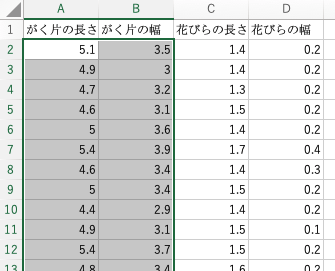
\includegraphics[width=5cm]{chap2/scatter_data.png}
        \caption{セルを選択した状態}
        \label{fig:scatter_data}
    \end{minipage}
 \begin{minipage}{0.5\hsize}
        \centering
        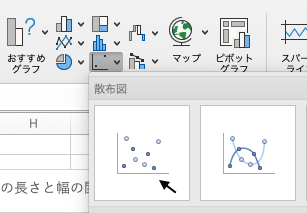
\includegraphics[width=6cm]{chap2/scatter_menu.png}
        \caption{散布図を選択する}
        \label{fig:select_barchart_hist}
    \end{minipage}
    \\
    \begin{minipage}{0.5\hsize}
        \centering
        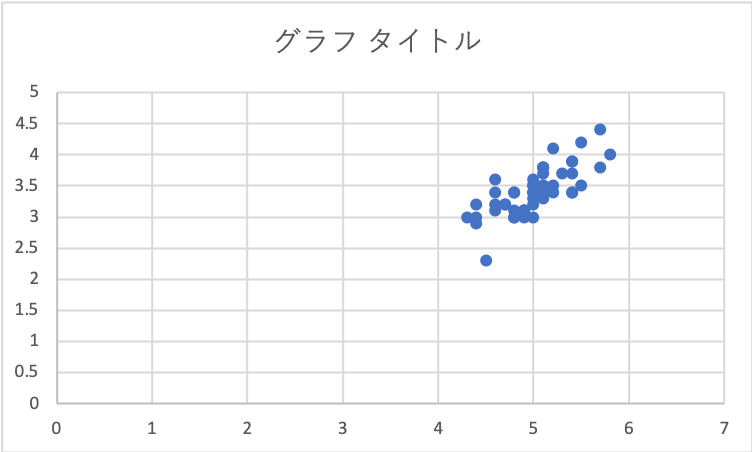
\includegraphics[width=6cm]{chap2/scatter1.png}
        \caption{未完成な散布図}
        \label{fig:scatter1}
    \end{minipage}
    \begin{minipage}{0.5\hsize}
        \centering
        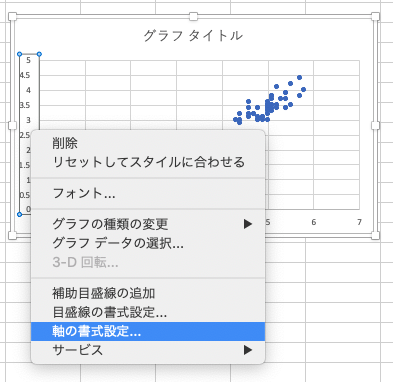
\includegraphics[width=4cm]{chap2/scatter_axis.png}
        \caption{軸のメニュー}
        \label{fig:scatter_axis}
    \end{minipage}
\end{figure}

\begin{figure}[tb]
    \begin{minipage}{0.5\hsize}
        \centering
        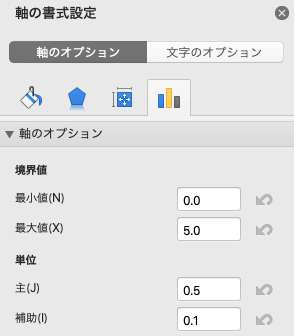
\includegraphics[width=4cm]{chap2/scatter_range.png}
        \caption{軸の範囲の設定}
        \label{fig:scatter_range}
    \end{minipage}
    \begin{minipage}{0.5\hsize}
        \centering
        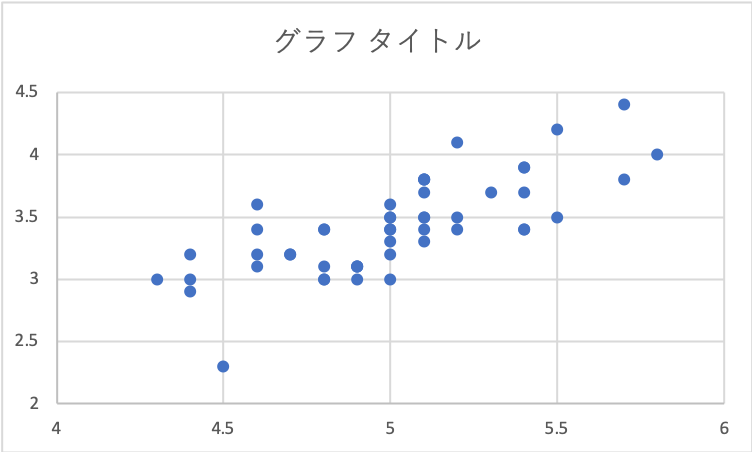
\includegraphics[width=6cm]{chap2/scatter2.png}
        \caption{軸の範囲を変えた散布図}
        \label{fig:scatter2}
    \end{minipage}
\end{figure}

\begin{figure}[tb]
    \begin{minipage}{0.5\hsize}
        \centering
        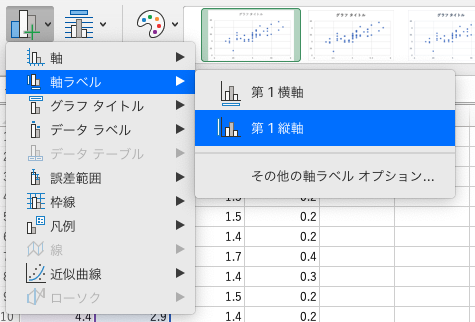
\includegraphics[width=5cm]{chap2/scatter_label.png}
        \caption{軸の範囲の設定}
        \label{fig:scatter_label}
    \end{minipage}
    \begin{minipage}{0.5\hsize}
        \centering
        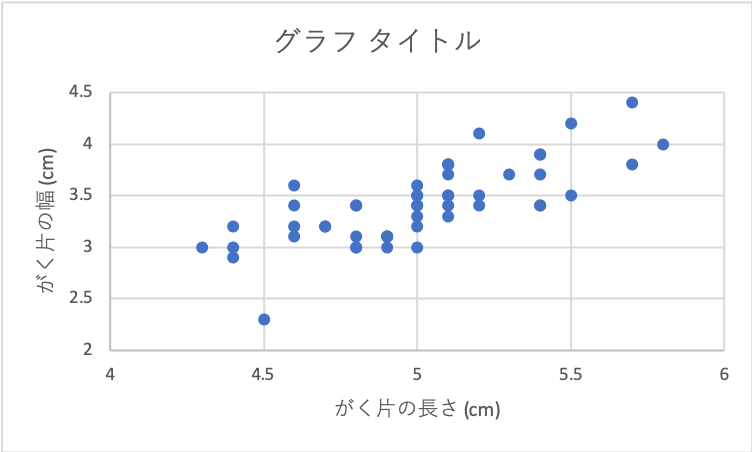
\includegraphics[width=6cm]{chap2/scatter3.png}
        \caption{軸のラベルを付けた散布図}
        \label{fig:scatter3}
    \end{minipage}
\end{figure}


\paragraph{演習}

csvファイルから散布図をかきなさい.ただし,横軸は 縦軸は にしなさい.

\subsection{相関係数}

Excelで相関係数を求めるのは簡単です.前回の総和を求めたのと同じ要領で行います.しかし,今回は2列データがありますので,そこだけ注意しましょう.

\begin{enumerate}
    \item 相関係数を入れるセルを選択します.
    \item ``=CORREL(''と入力します.
    \item 相関係数を求めたいデータの列を2つ選びます.
    \item ``)''と入力します.そうすると,相関係数が表示されます.
\end{enumerate}

\paragraph{演習}
csvデータから相関係数を求めなさい.

\subsection{回帰直線}

先程作成した散布図に回帰直線を追加します.

\begin{enumerate}
    \item リボンの``グラフのデザイン''を選びます.
    \item 図\ref{fig:regression_menu}のように,近似曲線の線形予測を選びます.
    そうすると,図\ref{fig:regression}のような回帰直線がかかれます.軸の範囲が変わった場合は,見やすいように変更しましょう.
\end{enumerate}

\begin{figure}[htbp]
    \centering
    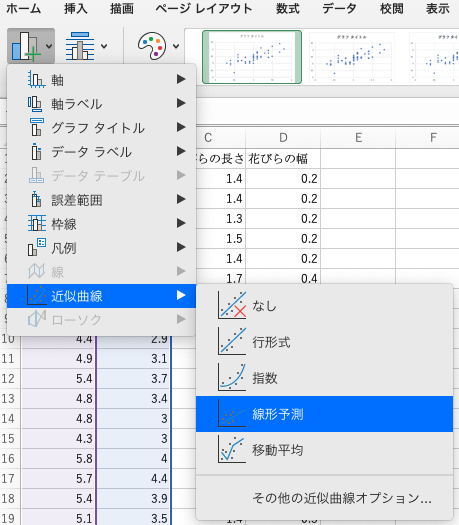
\includegraphics[width=6cm]{chap2/regression_menu.png}
    \caption{散布図}
    \label{fig:regression_menu}
\end{figure}

\paragraph{演習}

csvデータから回帰直線のかかれた散布図を作成しなさい.

\subsection{レポート提出}

レポートはkazuhisa.fujita@komatsu-u.ac.jpへ電子データとして提出する.データ形式はpdfとする.レポートの提出期限は次回の講義日までとする.

\section{おまけ}

R,python

プロット
R,matplotlib,gnuplot


有料ならmatlabがある.
